\subsection{Sensing Subsystem Testing}
\label{sec:sensing_subsystem_testing}

The Sensing subsystem will have each of its components tested on arrival, then components will be connected together to determine whether they are fit for the project. The components fit into two general categories, Electrical and Optical.

\paragraph{Electrical Optical Components:} 

\paragraph{Light Bulb} The tungsten light bulb produces a broad spectrum. The only optical information specified is that it produces 350 lumens. Lumens are a measure of brightness relative to human sight, and this is not usable for spectroscopy. The true power and spectral distribution of the bulb will be measured in an optical lab with a spectrometer and a power meter. The spectrometer fiber coupler will be set directly next to the bulb in a dark room and the light will be turned on and the spectral output captured. To measure the power, the bulb will be placed in a reflective enclosure and the power meter will be positioned to absorb output power. The results will be reported below.

Optical Power:

Spectral Output:

\paragraph{Photodetectors} The two photodetectors have light-current curves as displayed below.

\begin{figure}[H]
    \caption{Responsivity Diagrams for Testing}
    \centering
    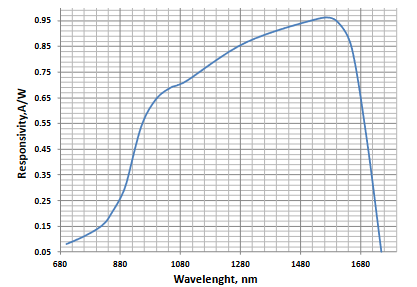
\includegraphics[width=0.5\textwidth]{images/InGaAsResponsivityCurve.png}
    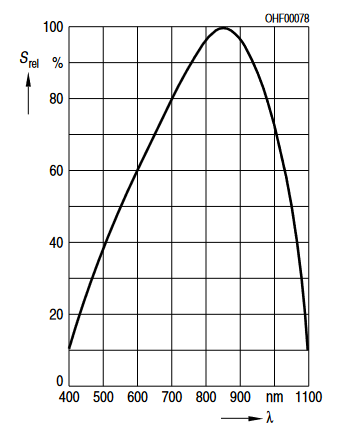
\includegraphics[width=0.5\textwidth]{images/NewarkBPX61.png}
\end{figure}

The diodes will be connected to a current meter and illumined with lasers at several wavelengths. Each laser will have its optical power measured by the same detector. The corresponding current will be reported below.

\begin{table}[H]
	\centering
	\label{table:VIS Diode Response}
	\bigskip
	\begin{tabular}{|p{2cm}|p{2.5cm}|p{2cm}|p{2.75cm}|}
	\hline
	Silicon Photodiode & Wavelength (nm) & Optical Power (W) & Generated Current (A)\\
	\hline
	Laser 1 & & & \\
	\hline
	Laser 2 & & & \\
	\hline
	Laser 3 & & & \\
	\hline
	\end{tabular}
\end{table}

\begin{table}[H]
	\centering
	\label{table:NIR Diode Response}
	\bigskip
	\begin{tabular}{|p{2cm}|p{2.5cm}|p{2cm}|p{2.75cm}|}
	\hline
	InGaAs Photodiode & Wavelength (nm) & Optical Power (W) & Generated Current (A)\\
	\hline
	Laser 1 & & & \\
	\hline
	Laser 2 & & & \\
	\hline
	Laser 3 & & & \\
	\hline
	\end{tabular}
\end{table}

\paragraph{Linear Actuator Rail} The linear actuator has three features that need to be verified on arrival, speed, power draw, and step size. 
\bigskip

A speed test will be conducted with the rail running along its entire stroke length while an observer records the time on a stopwatch device.
\bigskip

Speed (mm/s):
\bigskip

Power draw will be determined by running the linear actuator with no load. The actuator is rated for 0.8A current under no load. To test this, the actuator rail will be run through its full stroke length with a ammeter connected in series with its power line. An observer will record the total current draw.
\bigskip

Current Draw (A):
\bigskip

The step size of the rail is determined by the stepper motor step angle and the screw pitch. Based on its specs, this rail should have a step size of 0.005mm. In order to determine if this is the case, the rail will be taken through a set of 400 discrete steps, pausing rather than passing through them. A millimeter ruler will be fixed in place next to the rail plate to allow an observer to measure whether the total distance is 2mm.
\bigskip

400 Stroke Distance (mm):

\paragraph{Passive Optical Components:}

\paragraph{Fiber Patch Cable} The numerical aperture of the Fiber patch cable will be measured through trigonometry. An observer will collimate light into an optical fiber at one end and the other end they will place a flat surface a small distance away from the fiber output. By changing the distance to the surface and measuring the spot size, the numerical aperture can be approximated.
\bigskip

Fiber NA:
\bigskip

\paragraph{Fiber Collimator} The fiber collimator will have a similar test to determine its numerical aperture. A laser will be shone into one end of the optical system and a target surface will be placed nearby.
\bigskip

Collimator NA:
\bigskip

Incidentally, this is when the fiber and collimator will be tested together as well. The laser will be collimated into one end of the fiber and the beam will proceed out of the collimating lens on the other side. The beam diameter will be measured at 1 cm, 10cm and a meter to ensure sufficient collimation. The beam diameter should be no more than 2mm.
\bigskip

Beam Diameter at 1 cm (mm):	
Beam Diameter at 10 cm (mm):	
Beam Diameter at 1 m (mm):	

\paragraph{Focusing Lens} The focal length of the lens will be tested with a simple far field focus test. The observer will hold the optic low above a flat surface until images of the lighting overhead come into focus. The distance to the surface will be measured with an upright ruler.
\bigskip

Effective Focal Length (mm):
\bigskip

This value does not need to be known with exact certainty, the length of the carriage rail and the unbounded alignment distance add flexibility for this parameter.

\paragraph{Diffraction Grating} There are two parameters worth knowing from the diffraction grating. First we must check if it is the correct design. This will be done by setting it in the beam path of a laser and turning it 45 degrees so that the light interferes with the grooved surface. The angle will be checked to ensure that the groove count and blaze angle are correct. Next, the efficiency of the surface will be tested. This will be done by testing the laser power before and after hitting the surface. In order to increase the value of the measurement, optics will be added to expand the beam and make use of as much of the grating’s surface as possible.
\bigskip

Estimated Active Area (mm\^2):
Efficiency:

